\documentclass[11pt,a4paper]{article} % Prepara un documento con un font grande

\usepackage{iftex}

\ifLuaTeX
  % Adatta LaTeX alle convenzioni tipografiche italiane,
% e ridefinisce alcuni titoli in italiano, come "Capitolo" al posto di "Chapter",
% se il documento è in italiano
%\usepackage[italian]{babel}
%\usepackage[utf8]{inputenc} % Consente l'uso caratteri accentati italiani
%\usepackage{graphicx}		% Per le immagini
%\usepackage{gnuplot-lua-tikz}
%\usepackage[top=2.5cm, bottom=2cm, left=2cm, right=2cm]{geometry}

%\nonstopmode %non fermarti agli errori

%\usepackage{fancyhdr}
%\setlength{\headheight}{15.2pt}
%\pagestyle{fancy} % Solo le pagine normali, non i titoli nè la pagina iniziale


%%%%%%%%%%%%%%%%%%%%%%%%%%%%%%%%%%%%%%%%%%%%%%%%%%%%%%%%%%%%%%%%%%%%%%%%%%%%%%%%%%%%%%%%%

\usepackage{lipsum} % Package to generate dummy text throughout this template

\usepackage{fontspec}
\setmainfont[Ligatures=TeX]{Alegreya}

%\usepackage[sc]{mathpazo} % Use the Palatino font
%\usepackage[T1]{fontenc} % Use 8-bit encoding that has 256 glyphs
%%%%%
%\usepackage{Alegreya} %% Option 'black' gives heavier bold face 
%\renewcommand*\oldstylenums[1]{{\AlegreyaOsF #1}}

%\usepackage[euler-digits,euler-hat-accent]{eulervm}
%%%%%%
%\usepackage[utf8]{inputenc} % Consente l'uso caratteri accentati italiani
%\linespread{1.05} % Line spacing - Palatino needs more space between lines
\usepackage{amsmath, amsthm, amssymb, amsfonts}
\usepackage{microtype} % Slightly tweak font spacing for aesthetics

%%%%%%%%%%%%%%%%%%%%%%%%%%%%%%%%%%%%%%%%%%%%%
%Miei package
\usepackage[italian]{babel}
\usepackage{graphicx}		% Per le immagini
\usepackage{gnuplot-lua-tikz}
%%%%%%%%%%%%%%%%%%%%%%%%%%%%%%%%%%%%%%%%%%%%%
\usepackage[hmarginratio=1:1,top=32mm,columnsep=20pt]{geometry} % Document margins
\usepackage{multicol} % Used for the two-column layout of the document
\usepackage[hang, small,labelfont=bf,up,textfont=it,up]{caption} % Custom captions under/above floats in tables or figures
\usepackage{booktabs} % Horizontal rules in tables
\usepackage{float} % Required for tables and figures in the multi-column environment - they need to be placed in specific locations with the [H] (e.g. \begin{table}[H])
\usepackage{hyperref} % For hyperlinks in the PDF

\usepackage{lettrine} % The lettrine is the first enlarged letter at the beginning of the text
\usepackage{paralist} % Used for the compactitem environment which makes bullet points with less space between them

\usepackage{abstract} % Allows abstract customization
\renewcommand{\abstractnamefont}{\normalfont\bfseries} % Set the "Abstract" text to bold
\renewcommand{\abstracttextfont}{\normalfont\small\itshape} % Set the abstract itself to small italic text

\usepackage{titlesec} % Allows customization of titles
\renewcommand\thesection{\Roman{section}} % Roman numerals for the sections
\renewcommand\thesubsection{\Roman{subsection}} % Roman numerals for subsections
\titleformat{\section}[block]{\large\scshape\centering}{\thesection.}{1em}{} % Change the look of the section titles
\titleformat{\subsection}[block]{\large}{\thesubsection.}{1em}{} % Change the look of the section titles

\usepackage{fancyhdr} % Headers and footers
\pagestyle{fancy} % All pages have headers and footers
\fancyhead{} % Blank out the default header
\fancyfoot{} % Blank out the default footer
\fancyhead[C]{Running title $\bullet$ November 2012 $\bullet$ Vol. XXI, No. 1} % Custom header text
\fancyfoot[RO,LE]{\thepage} % Custom footer text


\else
  % Adatta LaTeX alle convenzioni tipografiche italiane,
% e ridefinisce alcuni titoli in italiano, come "Capitolo" al posto di "Chapter",
% se il documento è in italiano
%\usepackage[italian]{babel}
%\usepackage[utf8]{inputenc} % Consente l'uso caratteri accentati italiani
%\usepackage{graphicx}		% Per le immagini
%\usepackage{gnuplot-lua-tikz}
%\usepackage[top=2.5cm, bottom=2cm, left=2cm, right=2cm]{geometry}

%\nonstopmode %non fermarti agli errori

%\usepackage{fancyhdr}
%\setlength{\headheight}{15.2pt}
%\pagestyle{fancy} % Solo le pagine normali, non i titoli nè la pagina iniziale


%%%%%%%%%%%%%%%%%%%%%%%%%%%%%%%%%%%%%%%%%%%%%%%%%%%%%%%%%%%%%%%%%%%%%%%%%%%%%%%%%%%%%%%%%

\usepackage{lipsum} % Package to generate dummy text throughout this template

%\usepackage[sc]{mathpazo} % Use the Palatino font
\usepackage{tgpagella} % TeX Gyre Pagella, versione migliorata di Palatino. Si ma bo, no
%\usepackage{inconsolata} % Font monospace
\usepackage{textcomp}
\usepackage[scale=0.98,ttdefault]{AnonymousPro}

%%%%%
%\usepackage{Alegreya} %% Option 'black' gives heavier bold face 
\usepackage{AlegreyaSans} %% Option 'black' gives heavier bold face 
%\renewcommand*\oldstylenums[1]{{\AlegreyaOsF #1}}
%\usepackage{opensans}
%\usepackage[euler-digits,euler-hat-accent]{eulervm}
\usepackage[euler-hat-accent]{eulervm}
%%%%%%

\usepackage[T1]{fontenc} % Use 8-bit encoding that has 256 glyphs

\usepackage[utf8]{inputenc} % Consente l'uso caratteri accentati italiani
\linespread{1.08} % Line spacing - Palatino needs more space between lines, messo a 1.08 da 1.11 che era per alegreya
\usepackage{amsmath, amsthm, amssymb, amsfonts}
\usepackage[italian]{babel}
%\usepackage[kerning,spacing,tracking,letterspace = 2,babel]{microtype} % Slightly tweak font spacing for aesthetics. Il tre è pensato per Alegreya
\usepackage[kerning,spacing,babel]{microtype}
\SetTracking[]{encoding = *,shape = *}{3} % Aumenta la distanza fra le lettere
							     % http://tex.stackexchange.com/questions/66494/new-command-for-spacing-letters-in-microtype
%%%%%%%%%%%%%%%%%%%%%%%%%%%%%%%%%%%%%%%%%%%%%
%Miei package



\usepackage{graphicx}		% Per le immagini
\usepackage{fixltx2e}
%\usepackage{color}		% COLORI!

%\definecolor{grigio-molto-scuro}{gray}{0.1}	%colore

\usepackage{tabularx}		% Per le tabelle con le colonne tutte uguali
\usepackage{tabulary}		% Tabelle migliorate, nelle celle il testo va a capo da solo...
\usepackage{gnuplot-lua-tikz}
%%%%%%%%%%%%%%%%%%%%%%%%%%%%%%%%%%%%%%%%%%%%%
\newlength{\alphabet}
\settowidth{\alphabet}{\normalfont abcdefghijklmnopqrstuvwxyz}
\usepackage[
	    %hmargin=0.18\paperwidth,% metti la larghezza del testo (margini orizzontali) al 18% del foglio
	    textwidth=2.4\alphabet,  % http://tex.stackexchange.com/questions/59626/nicely-force-66-characters-per-line
	    hmarginratio=1:1,       % margini destro e sinistro uguali
	    top=35mm,	            % margine sopra a 32mm...
	    vmarginratio=4:5,       % quello sotto uguale (default 2:3)
	    columnsep=20pt]         % Spazio tra le colonne?
	    {geometry} % Document margins
\usepackage{multicol} % Used for the two-column layout of the document
\usepackage[hang, small,labelfont=bf,up,textfont=it,up]{caption} % Custom captions under/above floats in tables or figures
\usepackage{booktabs} % Horizontal rules in tables
\usepackage{float} % Required for tables and figures in the multi-column environment - they need to be placed in specific locations with the [H] (e.g. \begin{table}[H])
%\usepackage{tocloft} % Per customizzare le liste di floats (per i custom float!)
\usepackage[titles]{tocloft} %Pare causi meno casini con fancyhdr
\usepackage{nicefrac} % Per le frazioni tipo ⅛
\usepackage{pdfpages} % Per includere pagine intere in pdf (per la copertina)
%\usepackage[squaren]{siunitx}

\usepackage{lettrine} % The lettrine is the first enlarged letter at the beginning of the text
\usepackage{paralist} % Used for the compactitem environment which makes bullet points with less space between them
\usepackage[section]{placeins} % Per \FloatBarrier. L'opzione section comporta che le sezioni siano floatbarriers

\usepackage{abstract} % Allows abstract customization
\renewcommand{\abstractnamefont}{\normalfont\bfseries} % Set the "Abstract" text to bold
\renewcommand{\abstracttextfont}{\normalfont\small\itshape} % Set the abstract itself to small italic text

\usepackage{caption} % Per captions avanzate

\usepackage{listingsutf8} % Per includere codice sorgente meglio che con verbatim (e con caratteri non inglesi)
\lstset{ 
  %Preso anche questo da http://en.wikibooks.org/wiki/LaTeX/Source_Code_Listings
  %backgroundcolor=\color{white},   % choose the background color; you must add \usepackage{color} or \usepackage{xcolor}
  basicstyle=\footnotesize\ttfamily,        % the size of the fonts that are used for the code E MESSO IN MONOSPACE
  breakatwhitespace=true,         % sets if automatic breaks should only happen at whitespace
  breaklines=true,                 % sets automatic line breaking
  captionpos=b,                    % sets the caption-position to bottom
  %commentstyle=\color{mygreen},    % comment style
  %deletekeywords={...},            % if you want to delete keywords from the given language
  %escapeinside={\%*}{*)},          % if you want to add LaTeX within your code
  %extendedchars=true,              % lets you use non-ASCII characters; for 8-bits encodings only, does not work with UTF-8
  frame=l,                    % adds a frame around the code
				    %you can control the rules at the top, right, bottom, and left directly by using the four initial 
				    %letters for single rules and their upper case versions for double rules. http://mirror.hmc.edu/ctan/macros/latex/contrib/listings/listings.pdf
				    % Es frame frame=trBL ha doppia linea a sinistra e sotto, e singola a destra e sopra
  keepspaces=true,                 % keeps spaces in text, useful for keeping indentation of code (possibly needs columns=flexible)
  %keywordstyle=\color{blue},       % keyword style
  %language=Octave,                 % the language of the code
  %morekeywords={*,...},            % if you want to add more keywords to the set
  numbers=left,                    % where to put the line-numbers; possible values are (none, left, right)
  numbersep=5pt,                   % how far the line-numbers are from the code
  %numberstyle=\tiny\color{mygray}, % the style that is used for the line-numbers
  %rulecolor=\color{black},         % if not set, the frame-color may be changed on line-breaks within not-black text (e.g. comments (green here))
  showspaces=false,                % show spaces everywhere adding particular underscores; it overrides 'showstringspaces'
  showstringspaces=false,          % underline spaces within strings only
  showtabs=false,                  % show tabs within strings adding particular underscores
  stepnumber=1,                    % the step between two line-numbers. If it's 1, each line will be numbered
  %stringstyle=\color{mymauve},     % string literal style
  tabsize=2,                       % sets default tabsize to 2 spaces
  title=\lstname                   % show the filename of files included with \lstinputlisting; also try caption instead of title
}


\usepackage{titlesec} % Allows customization of titles
\renewcommand\thesection{\Roman{section}} % Roman numerals for the sections
\renewcommand\thesubsection{\Roman{subsection}} % Roman numerals for subsections
% \usefont {encoding} {family} {series} {shape}
\titleformat{\section}[block]{\AlegreyaSansSC \bfseries \LARGE}{\thesection.}{1em}{} % Change the look of the section titles. Pezzi spostati \scshape\centering\bfseries
\titleformat{\subsection}[block]{\AlegreyaSans \bfseries \Large}{\thesection.\thesubsection }{1em}{} % Change the look of the section titles

\usepackage{fancyhdr} % Headers and footers
\pagestyle{fancy} % All pages have headers and footers
\fancyhead{} % Blank out the default header
\fancyfoot{} % Blank out the default footer
\headheight=14pt % Perchè sennò continua a lamentarsi che 12pt è troppo poco e la mette a 14 lo stesso
%\fancyhead[C]{Chiappara, Labanca, Forcher - \textit{Ottica geometrica} $\bullet$ \thesection}
\fancyhead[L]{\textit{Ottica geometrica}} % Custom header text. \nouppercase{\leftmark} per sezione, ma non ci sta
\fancyhead[R]{\textsc{\nouppercase{\leftmark}}}
\fancyfoot[RO,LE]{\thepage} % Custom footer text

\usepackage[hidelinks]{hyperref} % For hyperlinks in the PDF
\hypersetup{
    bookmarks=true,         % show bookmarks bar?
    unicode=false,          % non-Latin characters in Acrobat’s bookmarks
   % pdftoolbar=true,        % show Acrobat’s toolbar?
   % pdfmenubar=true,        % show Acrobat’s menu?
   % pdffitwindow=false,     % window fit to page when opened
    %pdfstartview={FitH},    % fits the width of the page to the window
    pdftitle={Ottica geometrica},    % title
    pdfauthor={D. Chiappara, G. Labanca, F. Forcher},     % author
    pdfsubject={Relazione di ottica geometrica - Sperimentazioni II 2014},   % subject of the document
    %pdfcreator={Creator},   % creator of the document
    %pdfproducer={Producer}, % producer of the document
    pdfkeywords={ottica} {geometrica} {relazione} {Sperimentazioni}, % list of keywords
    %pdfnewwindow=true,      % links in new PDF window
    %colorlinks=false,       % false: boxed links; true: colored links
    linkcolor=red,          % color of internal links (change box color with linkbordercolor)
    citecolor=green,        % color of links to bibliography
    filecolor=magenta,      % color of file links
    urlcolor=cyan           % color of external links
}

\fi
\DeclareGraphicsExtensions{.pdf, .png, .jpg} % Se due immagini hanno lo stesso nome sceglile secondo l'ordine di filetype qui
\graphicspath{ {./img/} }					 % Path delle immagini 

\title{
\vspace{-2cm}
\fontsize{36pt}{10pt}\selectfont
RELAZIONE DI \\[8mm] ELETTRONICA \\[12mm]
Bozza di analisi dati
}
% \title{}
\author{
\large
\textsc{Francesco Forcher}\\[2mm]
\normalsize Università di Padova, Facoltà di Fisica\\
\normalsize francesco.forcher@studenti.unipd.it\\
\normalsize Matricola: \texttt{1073458}\\
\and
\large
\textsc{Davide Chiappara}\\[2mm]
\normalsize Università di Padova, Facoltà di Fisica\\
\normalsize davide.chiappara@studenti.unipd.it\\
\normalsize Matricola: \texttt{1070160}\\
\and
\large
\textsc{Gabriele Labanca}\\[2mm]
\normalsize Università di Padova, Facoltà di Fisica\\
\normalsize gabriele.labanca@studenti.unipd.it\\
\normalsize Matricola: \texttt{1069556}
}
\date{\today}

%%%%%%%%%%%%%%%%%%%%%%%%%%%%%%%%%%%%%%5%%%%%%%%%%%%%%%%%%%%%%%%%%%%%%%%%%%%%%%%%%%
%\usepackage{float}
%\usepackage{caption}
%\usepackage{multirow}
%\usepackage[top=3.6cm, bottom=1.5in, left=0.5in, right=0.5in]{geometry}

%%%%%%%%%%%%%%%%%
% Robe del package tocloft per fare gli indici delle mie tabelle e grafici
% texblog.org/2008/07/13/define-your-own-list-of/
%\newcommand{\listtabellaname}{Lista delle tabelle}
%\newlistof{tabella}{tab}{\listtabellaname}


%%%%%%%%%%%%%%%%%

% I miei stili di float, con le righe
\floatstyle{plaintop}
\newfloat{tabella}{tb}{lop} 
\floatname{tabella}{Tabella}

\floatstyle{ruled}
\newfloat{grafico}{tb}{loi} 
\floatname{grafico}{Grafico}

\newcommand{\tabellaautorefname}{\bfseries Tabella} % per \autoref del package hyperref
\newcommand{\graficoautorefname}{\bfseries Grafico} % Idem



%%%%%%%%%%%%%%%%%%%%%%%%%%%%%%%%%%%%%%%%%%%%%%%%%%%%%%%%%%%%%%%%%%%%%5%%%%%%%%%%%%%
% Comandi personalizzati

% \newcommand{\cm}{\,\mathrm{cm}}
% \DeclareMathOperator{\cov}{cov} % Covarianza
% \DeclareMathOperator{\var}{var} % Covarianza
% \newcommand{\mm}{\,\mathrm{mm}}
% \newcommand{\nm}{\,\mathrm{nm}}
% \newcommand{\usuq}{\nicefrac{1}{q}}
% \newcommand{\usup}{\nicefrac{1}{p}}



%////////////////////////////////////////////////////////////////////////////////////////////////////////////////////////////
%////////////////////////////////////////////////////////////////////////////////////////////////////////////////////////////
% Fine dei dati iniziali per il latex: il documento finale inizierà da qui
\begin{document}
{
\maketitle % Produce il titolo a partire dai comandi \title, \author e \date


% REGEX per modificare col textrm _\{([a-zA-Z0-9\,]{2,})\}   _{textrm{\1}}

\section{Misure dirette di resistenze}
I valori riportati in tabella (valori in $\Omega$) sono quelli delle misure dirette delle resistenze, prese col multimetro FLUKE 111; il fondo scala \`e di $200mA$ per le correnti e di $600mV$ per le tensioni.

%tabella RES DIRETTE
\begin{tabella}
	\centering
	\begin{center}
\begin{tabulary}{\textwidth}{CCC}
\toprule
Posizione relativa della lente & Diametro fascio a $30 \cm$ & Diametro fascio a $130 \cm$ \\ \midrule
0.400 & 1.187 & 1.000 \\ \midrule
0.450 & 1.193 & 1.105 \\ \midrule
0.460 & 1.171 & 1.172 \\ \midrule
0.475 & 1.168 & 1.190 \\ \midrule
0.500 & 1.186 & 1.254 \\ \midrule
0.550 & 1.190 & 1.367 \\
\bottomrule
\end{tabulary}
\end{center}

	\caption{Misure dirette resistenze}
	\label{tab:01_tab_1.tex}
\end{tabella}


Per stimare gli errori si \`e usata la formula seguente:
%formula diretta
\[ \sigma_R =0.58 \sqrt{ \sigma_{\textrm{sist}} + \sigma_{\textrm{stat}}}= 0.58 \sqrt{(R\cdot\Delta P + n_{\textrm{digit}} \cdot \min(\textrm{FS}))}\]
Infatti gli errori legati alla misurazione sono dovuti sia a errori di scala ($ R= k _R \cdot R^{(r)} $), sia a errori casuali connessi al numero di digit. Per chiarezza di notazione, $\sigma^{(r)}$ \`e considerato errore statistico, mentre con $\sigma$ si intende l'errore totale.

Per quanto riguarda le resistenze $R_5$ e $R_6$ in serie, da una misurazione diretta effettuata col multimetro FLUKE 111 risulta che $R_{\textrm{S,sper}}= (402 \pm 4 )\Omega$. Col calcolo teorico, il valore di tale resistenza equivalente risulta invece $R_{\textrm{S, teor}}=(402 \pm 2 )\Omega$, dove per l'errore teorico \`e stato considerato che $R_{\textrm{S,teor}}=k\cdot(R_1^{(r)} + R_2^{(r)})$, infatti la k \`e costante in misurazioni successive, mantenendo il medesimo fondo scala. Con semplice propagazione degli errori risulta che 
\[\sigma_{R_{\textrm{S,teor}}}=\sqrt{(R_1+R_2)^2\cdot\sigma_k^2+\sigma_{R_1^{(r)}}^2+\sigma_{R_2^{(r)}}^2}\]
dove $\sigma_k$ \`e stata ricavata dall'errore percentuale fornito dal costruttore del multimetro e considerando k distribuito uniformemente:
\(\sigma_k=0.58 \cdot Err\%\). 
\`E stata calcolata la correlazione tra le due diverse stime della resistenza, considerando che la loro differenza dovrebbe essere nulla:
\[\lambda=\frac{\left|(R_{\textrm{S,teor}}-R_{\textrm{S,sper}})-0\right|}{\sigma_{R_{\textrm{S,teor}}-R_{\textrm{S,sper}}}}=0.3\]
con $R_{\textrm{S,teor}}-R{S,sper}=k\cdot(R_{\textrm{S,sper}}^{(r)}-R_1^{(r)}-R_2^{(r)})$, da cui per propagazione si ricava che 
\[ \sigma_{R_{\textrm{S,teor}}} - \sigma{R_{\textrm{S,sper}}} = 
        \sqrt{ (R_{\textrm{S,teor}} -R_{\textrm{S,sper}})^2 \sigma_k^2 + 3 \sigma_R^{(r) 2} }\]

Per il calcolo della resistenza equivalente a $R_5$ e $R_6$ in parallelo, il valore misurato con il multimetro FLUKE 111 \`e $R_{\textrm{P,sper}}= (94 \pm 4) \Omega$.
Il valore teorico \`e $R_{\textrm{P,teor}}=(94 \pm 0.5) \Omega$: considerando che $R_{\textrm{P,teor}}=k  \frac{R_5^{(r)} R_6^{(r)}}{R_5^{(r)} + R_6^{(r)}}$ e propagando, riutilizzando la medesima semplificazione sull'errore di scala, si ottiene 
\[\sigma_{\textrm{P,teor}}=\sqrt{\left(\frac{R_5 R_6}{R_5+R_6}\right)^2 \sigma_k^2 + \frac{R_5^4 + R_6^4}{(R_5 + R_6)^4}  \sigma_{R_{\textrm{P,teor}}^{(r) 2}}} .\]
Per il calcolo della compatibilit\`a, si sono utilizzate le medesime formule che per le resistenze in serie, opportunamente adattate:
\[\lambda=
	\frac{ \left|(R_{\textrm{P,teor}}-R_{\textrm{P,sper}})-0 \right| } { \sigma_{R_{\textrm{P,teor}}}-\sigma_{R_{\textrm{P,sper}}}}=0.14.\] 

Nota bene: tutti i calcoli sono stati effettuati mantenendo un numero superiore di cifre significative, riducendone il numero solo in sede di presentazione dati.



 











\section{Misura voltamperometrica di una resistenza}
Per misurare una resistenza piccola \`e stato costruito un circuito come in figura (da aggiungersi). Una prima misura diretta \`e stata effettuata utilizzando il multimetro FLUKE 111, che \`e risultata $R_x=(3.0 \pm 0.1) \Omega$.
Costruito il circuito, si \`e variata la resistenza di carico e la potenza erogata dal generatore per indagare di quanto fosse la caduta di potenziale al variare della corrente che attraversa R. I dati ottenuti sono riportati in tabella. 

%tabella AMPERE-VOLT
\begin{tabella}
	\centering
	\begin{center}
\begin{tabulary}{\textwidth}{CC}
\toprule
i (mA) & V (mV) \\ \midrule
25.0 & 70.5 \\ \midrule
30.6 & 86.2 \\ \midrule
37.5 & 106.4 \\ \midrule
49.6 & 140.3 \\ \midrule
60.8 & 171.7 \\ \midrule
69.7 & 182.0 \\ \midrule
72.9 & 204.3 \\ \midrule
81.8 & 230.1 \\ \midrule
100.0 & 280.1 \\ \midrule
90.5 & 254.8 \\ 
\bottomrule
\end{tabulary}
\end{center}

	\caption{Misure caduta di potenziale}
	\label{tab:02_tab_1.tex}
\end{tabella}

In grafico sono riportate tali misure esprimendo V in funzione di I, sovrapposte a un fit lineare ottenuto col metodo della massima verosimiglianza.

\begin{grafico}
\centering
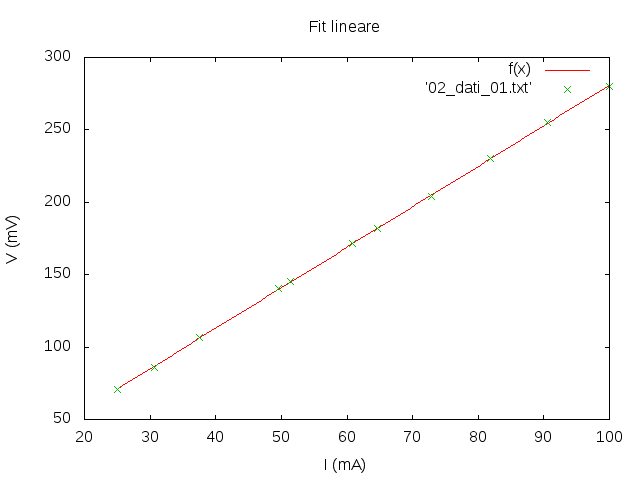
\includegraphics[width=\textwidth]{02_fitlin}
\caption{Fit lineare}
\label{fig:fitlin}
\end{grafico}

I coefficienti della retta interpolante $y=mx+c$ sono:
\[m = (2.809 \pm 0.004) \Omega \]
\[c = (0.2 \pm 0.2) mV.\]
%Calcolando la covarianza tra $m$ e $c$ si ottiene 
%\[cov(m, c) = -0.000660084 V^4\] %UDM
Si \`e calcolata la correlazione 
\[\rho(m, c) = \frac{cov(m, c)}{\sigma_m \sigma_c}=-0.11\]
e l'errore a posteriori sulla caduta di tensione \`e di $\sigma_V=0.6V$.

A seguire il grafico dei residui: si \`e rappresentata la differenza tra il valore di tensione misurato e quello ricavato teoricamente dalla retta interpolante in corrispondenza del suo valore di corrente.

\begin{grafico}
\centering
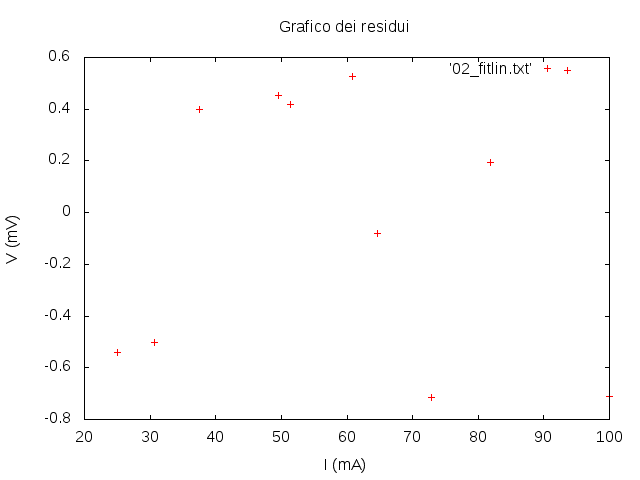
\includegraphics[width=\textwidth]{02_residui}
\caption{Residui}
\label{fig:residui}
\end{grafico}

Una stima della resistenza \`e data dalla pendenza della retta interpolante. Tale retta ha un errore che \`e composizione di un errore sistematico e di uno statistico, infatti si pu\`o scrivere $m=\frac{k_V (V_2^{(r)}-V_1^{(r)})}{k_i (i_2^{(r)} - i_1^{(r)})}=\frac{k_V}{k_i}m^{(r)}$.
Da una propagazione risulta che l'errore su tale grandezza \`e $\sigma_m=\sqrt{\sigma_{\textrm{m,fit}}^2 + \sigma_{k_V}^2 m^2 + \sigma_{k_i}^2 m^2}$ con $\sigma_{\textrm{m,fit}}$ errore casuale ottenuto dall'interpolazione.
Risulta che l'incertezza sulla resistenza \`e quasi completamente data dall'errore sistematico. Il risultato finale \`e $R=(2.8 \pm 0.4) \Omega$; l'errore percentuale \`e del $13 \%$.

Si possono confrontare il risultato teorico e quello sperimentale con un calcolo di compatibilit\`a. Dato che sono state usate strumentazioni differenti per le due stime, se ne pu\`o applicare la definizione: 
$\lambda=\frac{|R_x - R|}{\sqrt{\sigma_{R_x}^2+\sigma_R^2}}=0.5$.
 











\section{Resistenze interne degli strumenti di misura}
Attraverso costruzioni di circuiti o misure dirette, si sono stimate le resistenze interne degli strumenti utilizzati.
Per la stima della resistenza interna del generatore si \`e costruito un circuito come in figura (da aggiungersi) e utilizzato il voltmetro AGILENT U1232A con l'amperometro BECKMAN T110B.
Dalle misure risulta che
\begin{align}
V_0 &=(5.01 \pm 0.01 )V \ \textrm{con}\  V_{\textrm{FS}}=6V \\
i   &=(124.9 \pm 0.5) mA \ \textrm{con}\  i_{\textrm{FS}}=200mA \\
V   &=(5.00 \pm 0.01) V \ \textrm{con}\  V_{\textrm{FS}}=6V.
\end{align}
Da uno studio del circuito si ricava la formula $R_G=\frac{V_0-V}{V}$.
Stimandone l'errore, per evitare problemi di correlazione si pu\`o scrivere $R_G=\frac{k_v (V_0^{(r)}- V^{(r)})}{i}$, da cui propagando: 
\[\sigma_{R_G}=\sqrt{R_G^2 \sigma_{k_V}^2 + \frac{(\sigma_{V^{(r)}}^2 + \sigma_{V_0^{(r)}}^2)}{i^2} + \frac{(V_0-V)^2}{i^4} \sigma_i^2},\] ricordando che per $\sigma_i$ si intende l'errore strumentale totale. Concludendo, $R_G= (0.10 \pm 0.16) \Omega$.

Un diverso circuito \`e stato costruito per stimare la resistenza interna dell'AGILENT U1232A utilizzato come voltmetro.
Una misurazione diretta di $R_V$ \`e stata ottenuta utilizzando come ohmetro il BECKMAN T110B: $R_{\textrm{V, sper}}=(11.2 \pm 0.1) M\Omega$, con fondo scala di $20 M\Omega$. 
Le misure prese a circuito chiuso sono: 
\begin{align}
R_S &= (0.990 \pm 0.005) M\Omega \ \textrm{con}\  R_{\textrm{FS}}=6 M\Omega \\
V_0 &= (5.01 \pm 0.01) V \ \textrm{con}\  V_{\textrm{FS}} = 6 V \\
V &= (4.60 \pm 0.01) V \ \textrm{con}\  V_{\textrm{FS}} = 6 V
\end{align}
Studiando il circuito, si pu\`o dimostrare che 
\[ R_{\textrm{V, teor}} = \frac{R_S V}{V_0 - V} . \]
Portando fuori dai valori il coefficiente $k_V$ e semplificandolo, si ha $R_{\textrm{V, teor}} = \frac{R_S V^{(r)}}{V_0^{(r)} - V^{(r)}}$ da cui, propagando, si ottiene \[\sigma_{R_{\textrm{V,teor}}} = \sqrt{\sigma_{R_S}^2 \left(\frac{V}{(V_0 - V)^2} \right)^2 + \sigma_{V_{(r)}}^2 \left(\frac{R_S V_0}{(V_0 - V)^2}\right)^2 + \sigma_{V_0^{(r) 2}} \left(\frac{R_S V}{(V_0 - V)^2}\right)^2}.\]
Risulta $R_{\textrm{V, teor}} = (11.19 \pm 0.08) M\Omega$.


Per misurare la resistenza interna del BECKMAN T110B, usato come amperometro, si \`e semplicemente effettuato un collegamento con il FLUKE 111 usato come ohmetro. I valori sono riportati in tabella.

%tabella RESISTENZE AMPEROMETRO
\begin{tabella}
	\centering
	\begin{center}
\begin{tabulary}{\textwidth}{CCCC}
\toprule
$I_{FS}$ & $R (\Omega)$ & $\sigma_R (\Omega)$ & $R_{FS} (\Omega)$ \\ \midrule
200 mA & 1002 & 5 & 6000 \\ \midrule
2 mA & 102.1 & 0.5 & 600 \\ \midrule
20 mA & 11.4 & 0.1 & 600 \\ \midrule
200 mA & 1.8 & 0.1 & 600 \\ \midrule
2 A & 1.2 & 0.1 & 600 \\ 
\bottomrule
\end{tabulary}
\end{center}

	\caption{Resistenze dell'amperometro BECKMAN}
	\label{tab:03_tab_1.tex}
\end{tabella}


























\end{document}
